% ============================================
% Chapitre 5 : Configuration des Agents
% ============================================
\chapter{Configuration des Clients (Agents)}
\label{chap:agents}

\section{Vue d'Ensemble}

Les agents Zabbix sont des logiciels installés sur les machines à superviser. Ils collectent les métriques système et les transmettent au serveur Zabbix.

\begin{table}[H]
\centering
\caption{Modes de communication des agents}
\label{tab:agent-modes}
\begin{tabular}{|l|p{10cm}|}
\hline
\textbf{Mode} & \textbf{Description} \\
\hline
Passif & Le serveur interroge l'agent (port 10050) \\
\hline
Actif & L'agent envoie les données au serveur (port 10051) \\
\hline
\end{tabular}
\end{table}

\section{Installation sur Linux (Ubuntu)}

\subsection{Connexion au Client Linux}

\begin{lstlisting}[language=bash, caption=Connexion SSH au client Linux]
ssh -i "votre-cle.pem" ubuntu@<IP-CLIENT-LINUX>
\end{lstlisting}

\subsection{Installation de l'Agent Zabbix}

\begin{lstlisting}[language=bash, caption=Installation de l'agent Zabbix sur Ubuntu]
# Telecharger le package Zabbix
wget https://repo.zabbix.com/zabbix/7.0/ubuntu/pool/main/z/\
zabbix-release/zabbix-release_latest_7.0+ubuntu22.04_all.deb

# Installer le package
sudo dpkg -i zabbix-release_latest_7.0+ubuntu22.04_all.deb

# Mettre a jour et installer l'agent
sudo apt update
sudo apt install -y zabbix-agent
\end{lstlisting}

\subsection{Configuration de l'Agent Linux}

Éditer le fichier de configuration :

\begin{lstlisting}[language=bash, caption=Édition de la configuration]
sudo nano /etc/zabbix/zabbix_agentd.conf
\end{lstlisting}

Modifier les paramètres suivants :

\begin{lstlisting}[caption=Configuration zabbix\_agentd.conf (Linux)]
# Adresse IP du serveur Zabbix (IP privee)
Server=10.0.1.X

# Pour le mode actif
ServerActive=10.0.1.X

# Nom d'hote (doit correspondre dans Zabbix)
Hostname=ELBadry-Client-Linux

# Autoriser les commandes a distance (optionnel)
EnableRemoteCommands=1
\end{lstlisting}

\begin{figure}[H]
\centering
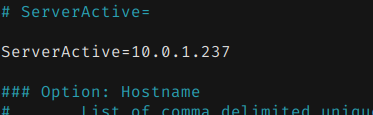
\includegraphics[width=0.95\textwidth]{images/20-agent-linux-configuration.png}
\caption{Configuration de l'agent Zabbix sur Linux}
\label{fig:agent-linux-config}
\end{figure}

\subsection{Démarrage du Service}

\begin{lstlisting}[language=bash, caption=Démarrage de l'agent Linux]
# Redemarrer l'agent
sudo systemctl restart zabbix-agent

# Activer au demarrage
sudo systemctl enable zabbix-agent

# Verifier le statut
sudo systemctl status zabbix-agent
\end{lstlisting}

\subsection{Vérification de la Connectivité}

\begin{lstlisting}[language=bash, caption=Test de connectivité]
# Verifier que l'agent ecoute sur le port 10050
sudo netstat -tlnp | grep 10050

# Tester la connexion depuis le serveur Zabbix
zabbix_get -s <IP-CLIENT-LINUX> -k agent.ping
\end{lstlisting}

\section{Installation sur Windows}

\subsection{Connexion RDP}

Se connecter au client Windows via Remote Desktop :
\begin{enumerate}
    \item Ouvrir \texttt{mstsc.exe}
    \item Entrer l'IP publique du client Windows
    \item Utiliser les credentials récupérés (Administrator)
\end{enumerate}

\begin{figure}[H]
\centering
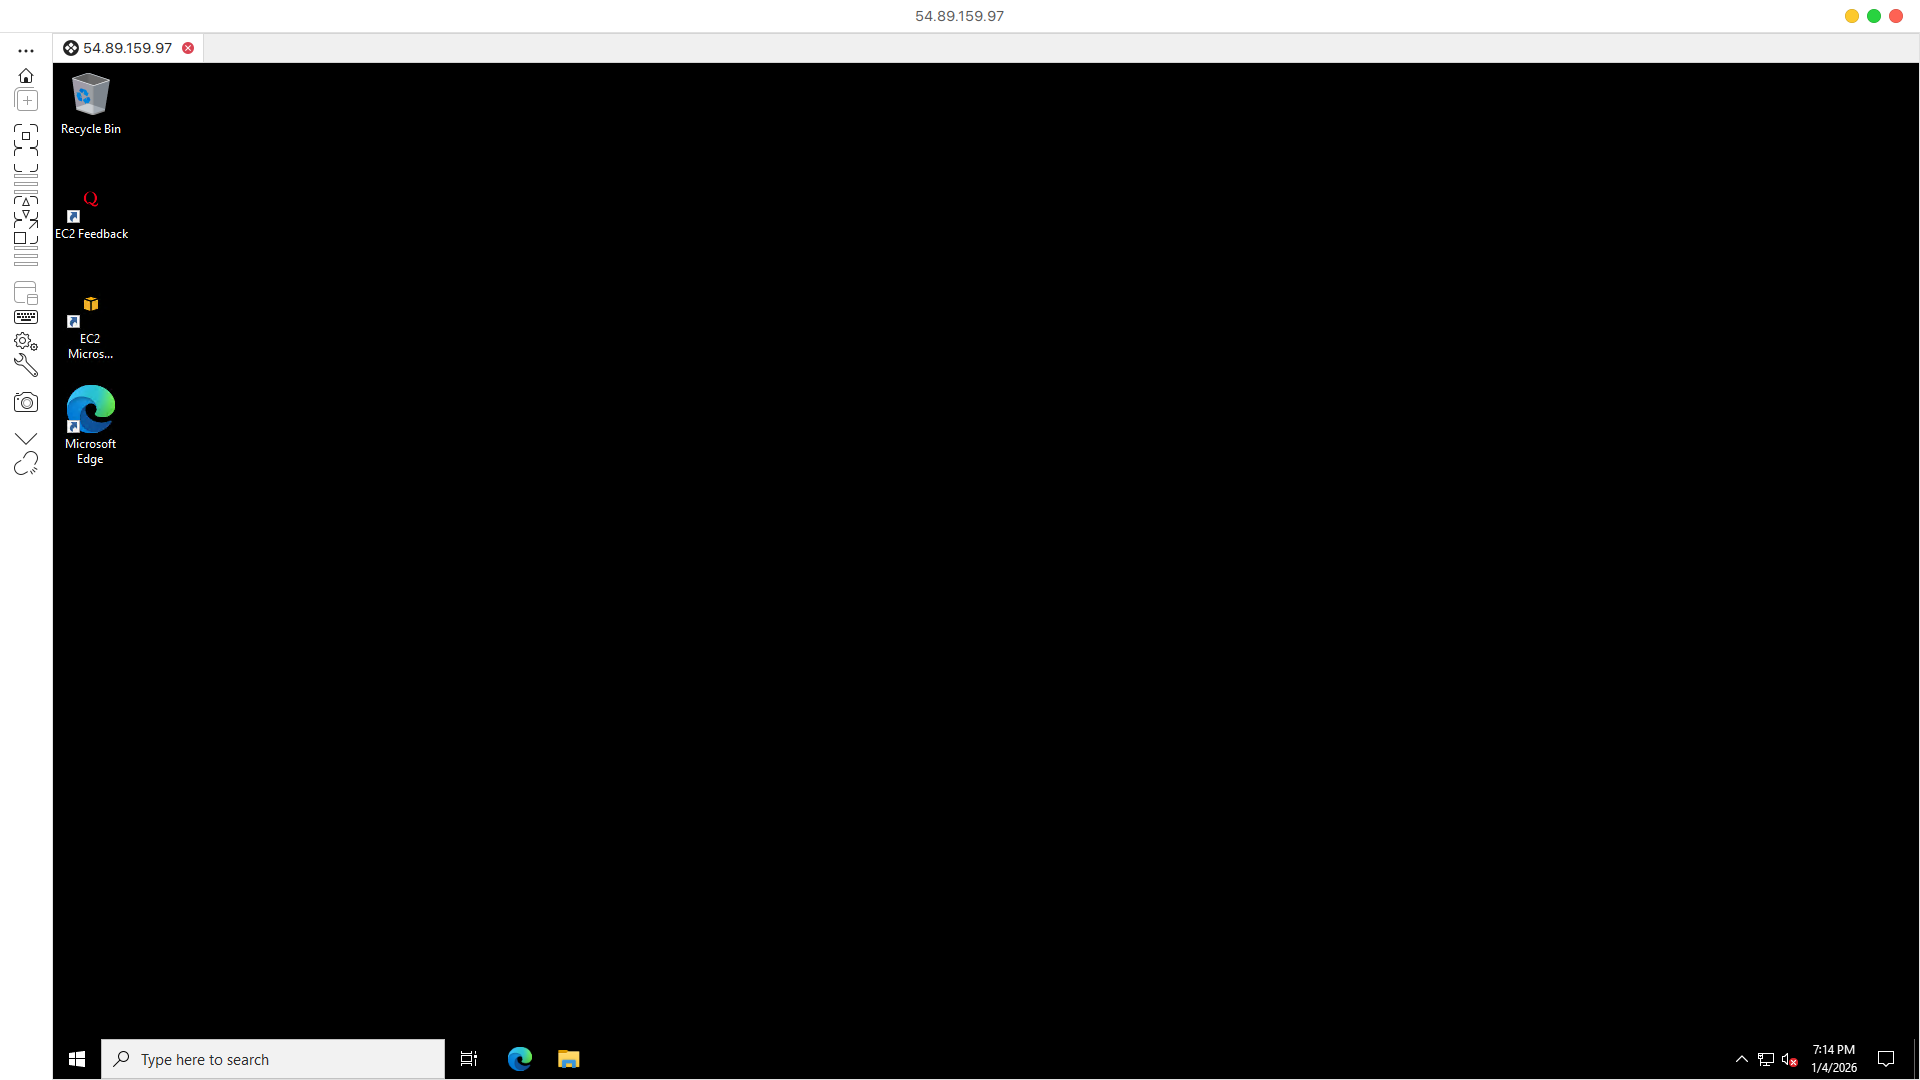
\includegraphics[width=0.85\textwidth]{images/21-windows-rdp-connection.png}
\caption{Connexion RDP au client Windows}
\label{fig:windows-rdp}
\end{figure}

\subsection{Téléchargement de l'Agent}

\begin{enumerate}
    \item Ouvrir le navigateur sur le serveur Windows
    \item Aller sur : \url{https://www.zabbix.com/download_agents}
    \item Sélectionner :
    \begin{itemize}
        \item OS : Windows
        \item Version : 7.0 LTS
        \item Architecture : AMD64
        \item Format : MSI
    \end{itemize}
    \item Télécharger le fichier MSI
\end{enumerate}

\subsection{Installation de l'Agent Windows}

\begin{enumerate}
    \item Exécuter le fichier MSI téléchargé
    \item Configurer les paramètres :
    \begin{itemize}
        \item \textbf{Zabbix Server IP} : IP privée du serveur (10.0.1.X)
        \item \textbf{Agent Hostname} : ELBadry-Client-Windows
        \item \textbf{Listen Port} : 10050
    \end{itemize}
    \item Terminer l'installation
\end{enumerate}

\begin{figure}[H]
\centering
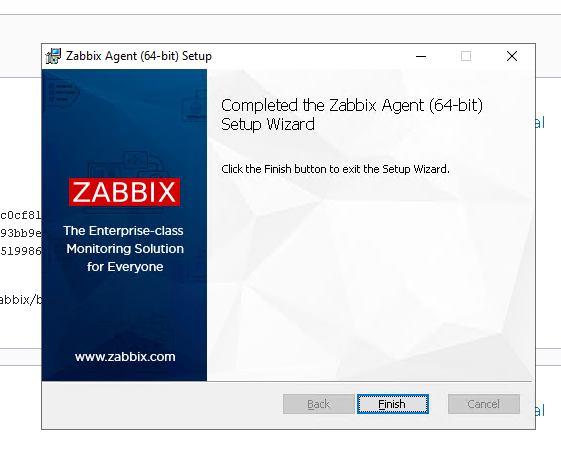
\includegraphics[width=0.85\textwidth]{images/22-agent-windows-installation.png}
\caption{Installation de l'agent Zabbix sur Windows}
\label{fig:agent-windows-install}
\end{figure}

\subsection{Vérification du Service Windows}

\begin{enumerate}
    \item Ouvrir \texttt{services.msc}
    \item Rechercher "Zabbix Agent"
    \item Vérifier que le service est en état "Running"
\end{enumerate}

\subsection{Configuration du Pare-feu Windows}

S'assurer que le port 10050 est ouvert :

\begin{enumerate}
    \item Ouvrir Windows Firewall
    \item Créer une règle entrante pour le port TCP 10050
    \item Autoriser les connexions
\end{enumerate}

\section{Ajout des Hôtes dans Zabbix}

\subsection{Ajouter le Client Linux}

\begin{enumerate}
    \item Dans Zabbix Web : \textbf{Data collection → Hosts → Create host}
    \item Configurer :
    \begin{itemize}
        \item \textbf{Host name} : ELBadry-Client-Linux
        \item \textbf{Groups} : Linux servers
        \item \textbf{Interfaces} : Agent, IP = 10.0.1.X, Port = 10050
    \end{itemize}
    \item Dans l'onglet \textbf{Templates} : Ajouter "Linux by Zabbix agent"
    \item Cliquer sur \textbf{Add}
\end{enumerate}

\begin{figure}[H]
\centering
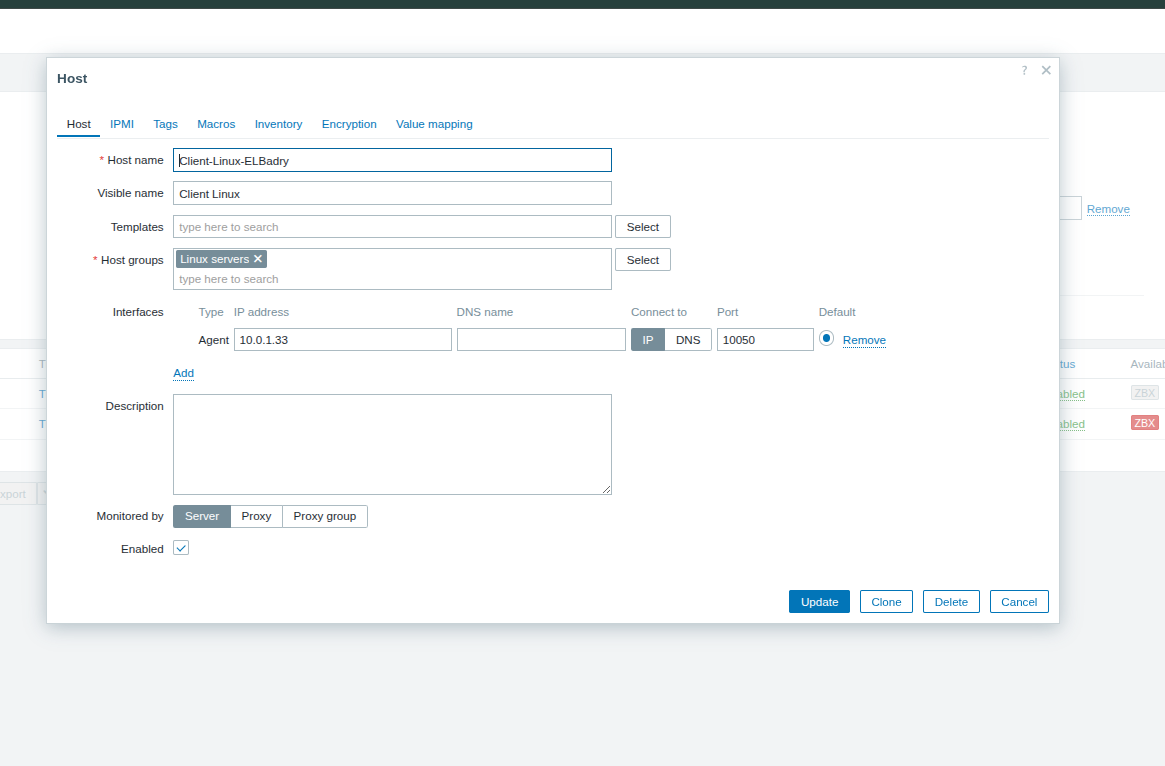
\includegraphics[width=0.95\textwidth]{images/23-zabbix-add-host-linux.png}
\caption{Ajout du client Linux dans Zabbix}
\label{fig:add-host-linux}
\end{figure}

\subsection{Ajouter le Client Windows}

\begin{enumerate}
    \item \textbf{Data collection → Hosts → Create host}
    \item Configurer :
    \begin{itemize}
        \item \textbf{Host name} : ELBadry-Client-Windows
        \item \textbf{Groups} : Windows servers (créer si nécessaire)
        \item \textbf{Interfaces} : Agent, IP = 10.0.1.X, Port = 10050
    \end{itemize}
    \item Dans l'onglet \textbf{Templates} : Ajouter "Windows by Zabbix agent"
    \item Cliquer sur \textbf{Add}
\end{enumerate}

\section{Vérification de la Connexion}

\subsection{Liste des Hôtes}

\begin{figure}[H]
\centering
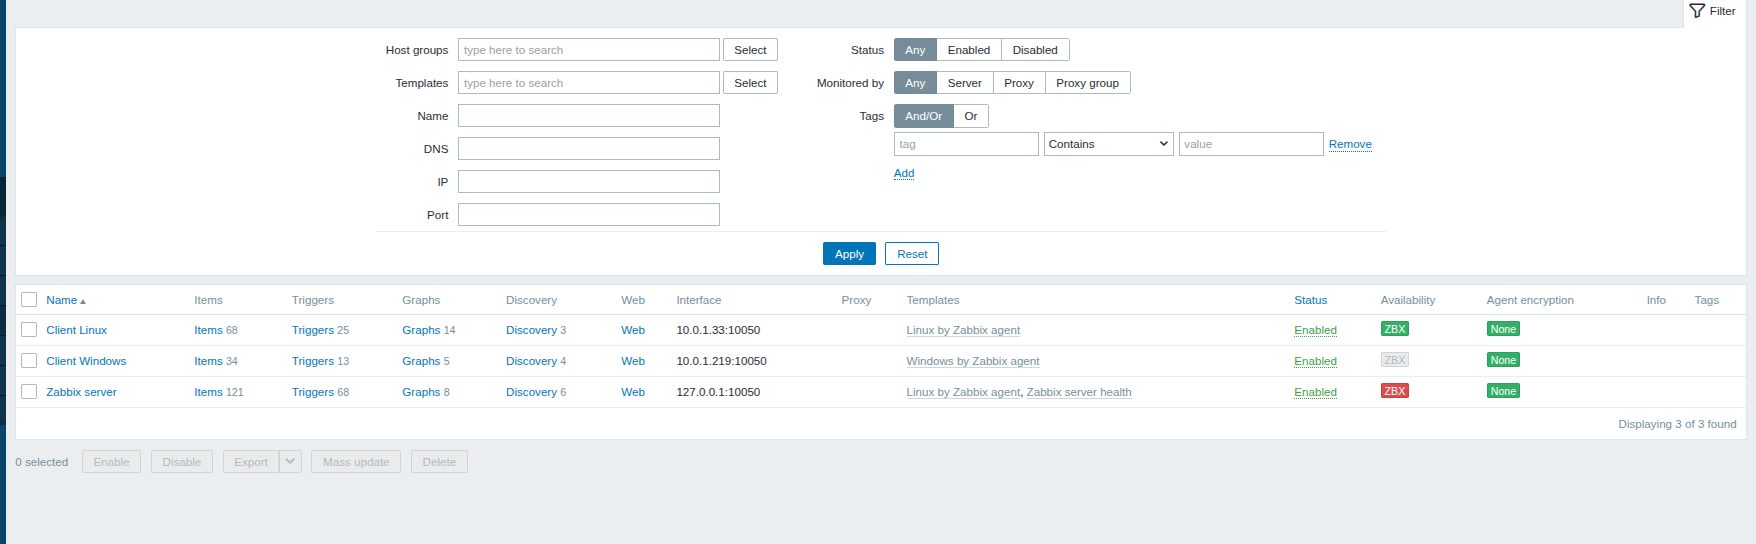
\includegraphics[width=0.95\textwidth]{images/24-zabbix-hosts-list.png}
\caption{Liste des hôtes configurés dans Zabbix}
\label{fig:hosts-list}
\end{figure}

\subsection{Statut des Agents (ZBX Vert)}

Le statut "ZBX" vert indique que l'agent est correctement connecté et répond aux requêtes du serveur.

\begin{figure}[H]
\centering
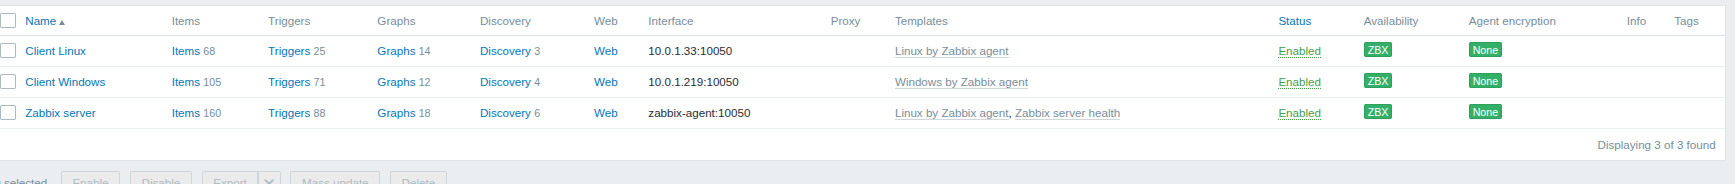
\includegraphics[width=0.95\textwidth]{images/25-zabbix-hosts-status-green.png}
\caption{Statut ZBX vert - Agents connectés avec succès}
\label{fig:zbx-green}
\end{figure}

\section{Tableau Récapitulatif des Agents}

\begin{table}[H]
\centering
\caption{Configuration des agents}
\label{tab:agents-config}
\begin{tabular}{|l|c|c|}
\hline
\textbf{Propriété} & \textbf{Client Linux} & \textbf{Client Windows} \\
\hline
Hostname & ELBadry-Client-Linux & ELBadry-Client-Windows \\
\hline
IP Privée & 10.0.1.X & 10.0.1.X \\
\hline
Port & 10050 & 10050 \\
\hline
Template & Linux by Zabbix agent & Windows by Zabbix agent \\
\hline
Version Agent & 7.0 & 7.0 \\
\hline
\end{tabular}
\end{table}
